\section{Platform Isolation Environment}
\label{sec:approach}

In this section, we describe platform isolation environment or \name in detail. \name is based on the idea of \nameenclave{}s that integrates \sphw devices to the traditional processor-core enclaves while maintaining small hardware and software TCB. First, we discuss the changes needed to incorporate into the \sphw to make them compatible with \name. Then we introduce a shared memory model that allows enclaves to communicate with each other and \sphw securely. Next, we discuss how the enclave life cycle changes given these modifications and how a remote verifier can get proof of the state of a \nameenclave{}. Finally, we provide a software design for \name that makes \name for the software developers easy to adapt.


% \begin{figure}[t]
%     \centering
%     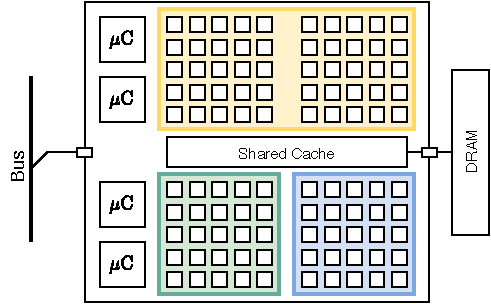
\includegraphics[width=0.8\linewidth]{images/accelerator.pdf}
%     \caption{Example of a TEE on an accelerator with multiple enclaves running simultaneously while being isolated from each other. In this example, there are three distinct enclaves running on a subset of the compute units of the accelerator indicated by a yellow, green, and blue overlay.}
%     \label{fig:accelerator}
% \end{figure}

\subsection{Changes to \sphw} There exists a wide range of \sphw{} devices that have unique behavior and integrate differently into \name{}.  In this chapter, we try to cover most devices but stress that some special cases require further analysis. We go from the simplest \sphw device we can imagine, a simple sensor, to one of the most complex, a sophisticated accelerator for a data center. Most other \sphw devices should fall in between these two examples and thus may require modifications between these two extremes. 

\begin{enumerate}
\item\emph{Simple Sensors} e.g., a temperature sensor only requires a minimal form of attestation to be integrated into \name{}. They must contain some key materials to sign some statements about themselves. This is mandatory for (remote) attestation of a \nameenclave that includes an attestation report of such a sensor. Usually, these sensors do not contain any secret data from a processor-local enclave and hence do not need to protect such data.

\item\emph{Accelerators} on the other hand, tend to be very complex and require more extensive modifications. Like the former, they must support attestation, but they may also support isolation for multiple enclaves' secret data. Let us assume data-center applications, where multiple stakeholders want to move multiple compute-intensive tasks from the CPU to the accelerator. The individual tasks' data should remain confidential and isolated, not only on the CPU but also on the accelerator. Thus, such an accelerator requires isolated and attestable domains -- in other words -- enclaves that run on the \sphw. 

\end{enumerate}

%\subsection{Communication with \sphw}
%\label{sec:system:comm}

%Platforms with a diverse set of \sphw are usually complex. Specifically, \sphw are connected to the processor over buses, which are, in turn, controlled by bus controllers as shown in \Cref{fig:bus}. This section describes how \sphw and processor-local enclaves can communicate in a secure way. As mentioned in \Cref{sec:overview}, \sphw communicate communicate over memory mapped address ranges either in the form of MMIO registers or DMA memory regions. To isolate these address regions we rely on existing hardware mechanisms, mainly PMP.
%Until now such hardware mechanisms have predominantly been used to restrict access to memory, but they can also be used to restrict access to any other address that is not in the DRAM range. The specific address ranges and model numbers of \sphw are described in a format called device tree. The device tree tells the OS, or any software during boot, where it can find which \sphw. It is usually stored in on-chip ROM and is provided to the OS by a zero-stage boot-loader, and thus, it can be considered trusted. The SM has access to this specification and can verify that only one specific enclave can access the correct address range for a certain \sphw. This limits the number of enclaves per bus type to one, e.g., only a single enclave can access all devices connected to the SPI bus at once. 

%\Sphw and buses that are used in a direct memory access (DMA) fashion behave differently. Such devices usually first negotiate a shared memory range through memory mapped registers. The established shared memory range is then used for all future communication. 
%For these \sphw, our proposal must support shared memory between an enclave and a \sphw.
%However, the DMA region can be established by an untrusted source, e.g., the OS. Therefore, the shared memory region supplied to the SM from the untrusted OS must be verified to detect any manipulation attempts. In our design, the SM verifies this in by performing an initial attestation to the \sphw and to its DMA configuration.

\subsection{Shared memory}
\label{sec:approach:sharedMemory}
Shared memory is a common mechanism for software to communicate across multiple cores or DMA regions of a \sphw. In our prototype, shared memory regions are centrally maintained by the CPU to enforce isolation as all \sphw is connected to the CPU.


\begin{enumerate}
\item\emph{Shared Memory between Processor-local Enclaves}
As mentioned before, processor-local enclaves rely on PMP entries for isolation. We reuse the functionality of PMPs also to protect shared memory regions. Therefore, our proposal does not require any changes to the processor itself, as PMP is already part of the RISC-V standard~\cite{riscv2019privspec}, and thus, it is already part of many processors. The SM, however, requires some modifications. For example, to store the configuration details for every shared memory region in local memory, the SM needs to reconfigure the PMP entries on a context switch similar to stock Keystone. It also must guarantee that at most two entities have access to the same shared buffer at a time. Additionally, the SM flushes the buffers' content when one enclave is destroyed not to leak stale data. 


\item\emph{Shared Memory with \sphw} \Sphw are connected to the CPU over buses, which are, in turn, controlled by bus controllers. As mentioned in \Cref{sec:overview}, \sphw communicate over memory-mapped address ranges either in the form of MMIO registers or DMA memory regions. To isolate these address regions, we rely on existing hardware mechanisms, mainly PMP. Until now, such hardware mechanisms have predominantly been used to restrict memory access, but they can also be used to restrict access to any other address that is not in the DRAM range. Our prototype reuses the concepts from shared memory between processor-local enclaves by assuming the \sphw to be another processor-local enclave. As such, it can directly share an address range with a real processor-local enclave. The SM represents a \sphw internally as a special case of a processor-local enclave that cannot be scheduled or called, but it may share some address regions with other enclaves. 

\end{enumerate}

% \begin{figure}[tbp]
%     \centering
%      \includestandalone[width=\linewidth]{images/tikz/lifecycle}
%     \caption{\textbf{The lifecycle of platform-wide enclaves.} The differences to traditional enclaves is highlighted in green. Note that, asynchronous disconnects can happen in all three possible states.\moritz{todo: beautify, or maybe change completely}}
%     \label{fig:lifecycle}
% \end{figure}


% \begin{figure}[t]
%   \centering
%   %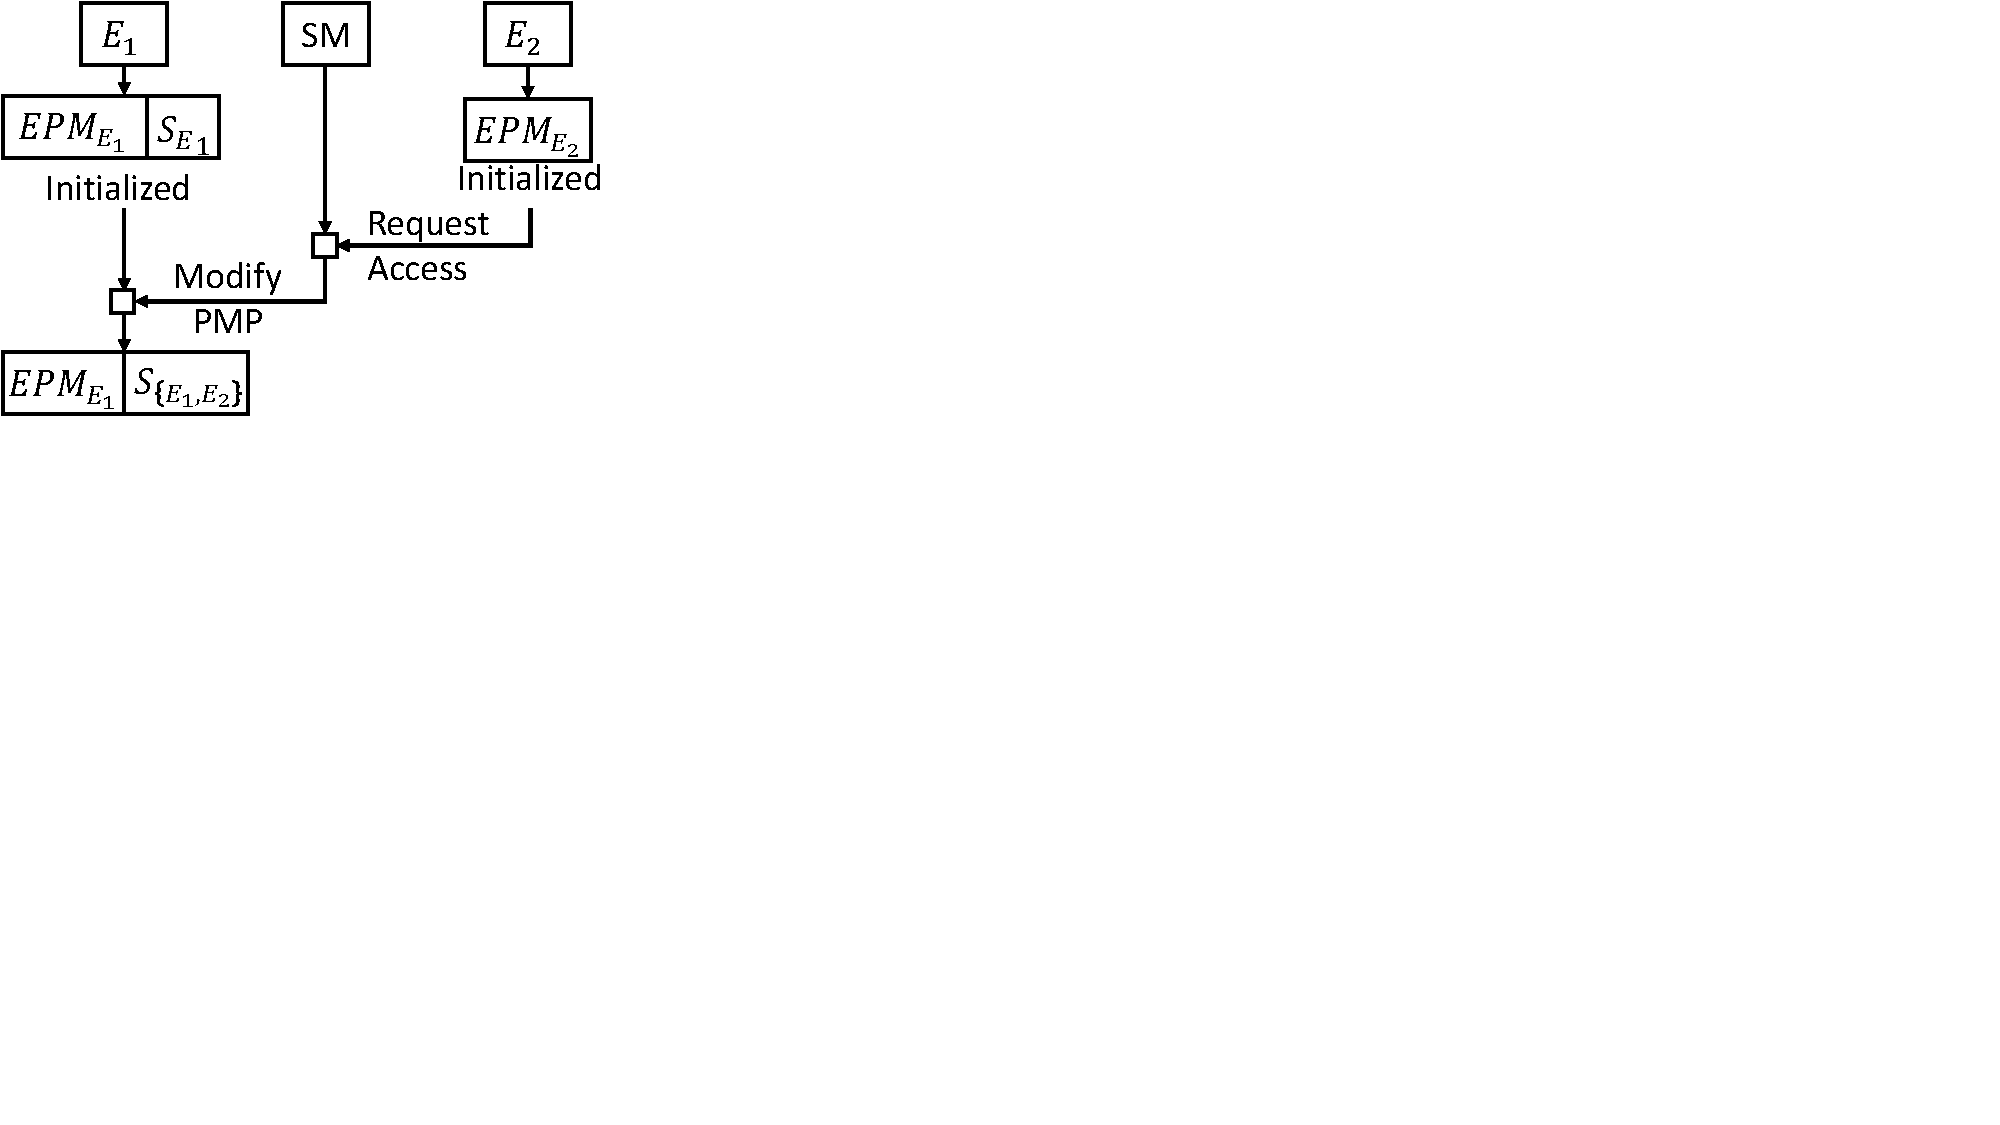
\includegraphics[trim={0 12cm 23cm 0}, clip, width=0.65\linewidth]{sharedMemoryInit.pdf}
%   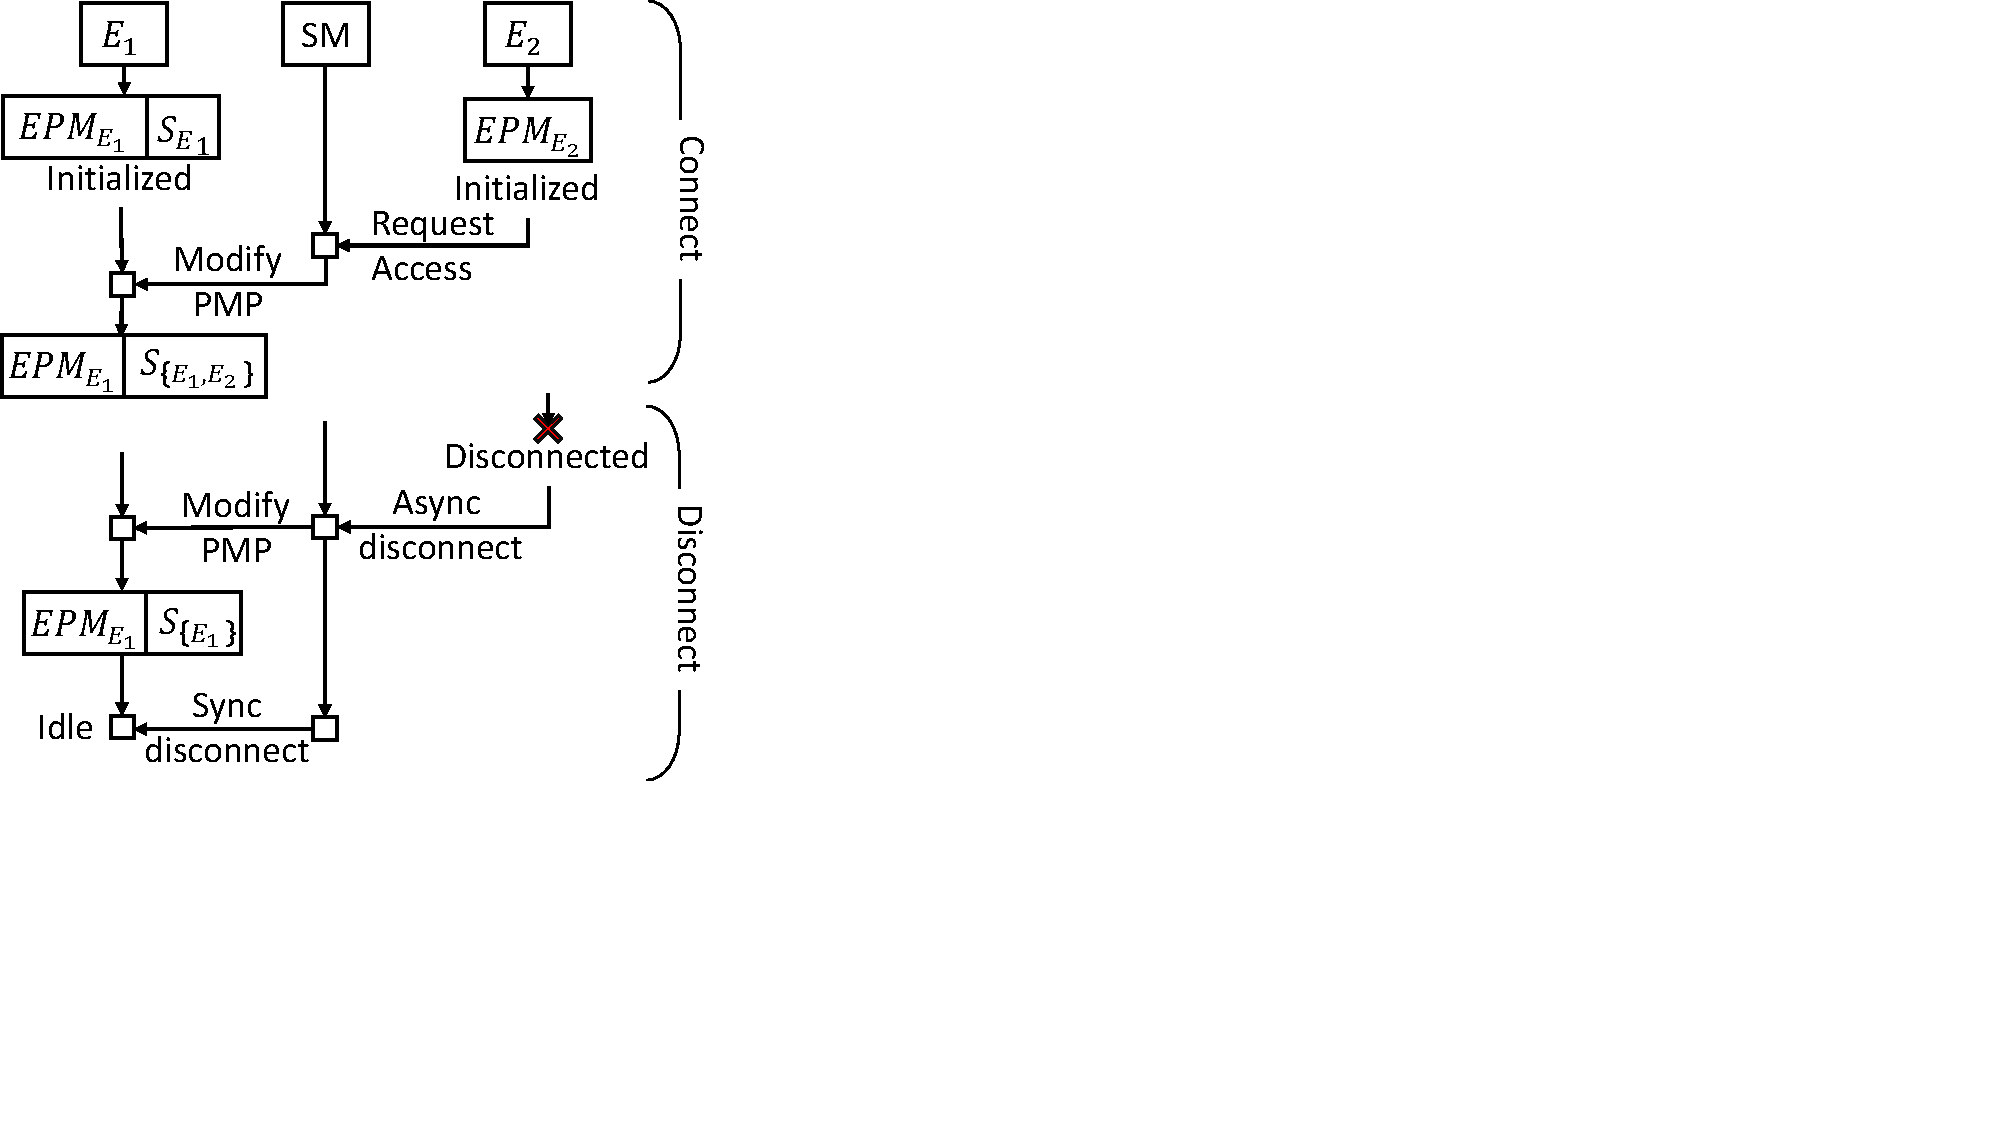
\includegraphics[trim={0 5.4cm 22cm 0}, clip, width=0.65\linewidth]{lifeCycle.pdf}
%   \vspace{-1em}
%   \caption{The life-cycle events of two example enclaves $E_1$ and $E_2$. $EPM_{E_1}$ and $EPM_{E_2}$ denote the enclave private memory (EPM) regions of $E_1$ and $E_2$ respectively. $S$ stands for the shared memory region and the subscript denotes the enclave(s) it is shared between. The security monitor (SM) acts as the intermediary in the \texttt{connect} and \texttt{disconnect} events.} \vspace{-1.2em}
%   \label{fig:sharedmemexample}
% \end{figure}

\myparagraph{Polling and Interrupts}
\sphw are synchronized with the processor with either polling or interrupts. Polling requires the CPU to check at a predetermined rate if new data is available from the \sphw, and thus, it can immediately be used in \name{}. On the other hand, interrupts are more complicated as they enable the \sphw to notify the CPU that new data is available with the processor's hardware support. In RISC-V specifically, interrupts can be delegated from the highest privilege mode to lower ones. So, in our prototype of \name{}, the SM can delegate individual types of interrupts either to an enclave or to the OS\footnote{In RISC-V external interrupts are handled by the platform interrupt controller (PLIC) and then multiplexed on top of the external interrupt signals to the core. Thus the SM has to contain a driver for the PLIC to figure out which \sphw the interrupt is from.}. Therefore, enclaves could also contain interrupt-handlers to, e.g., handle interrupts for a specific \sphw. Note that in our prototype, we only focus on polling. 

\subsection{Enclave life cycle}
\label{sec:lifeycle}

Traditional enclave's life cycle includes three distinct states: idle, running, and paused. E.g., the enclave is first created and started in the idle state. Then the enclave transitions to the running state after a call from a user. Due to a timer interrupt by the OS scheduler, it is paused. It resumed again as soon as the scheduler yields back to the enclave. 

\myparagraph{Attaching \sphw}
Before going into the lifecycle details, it is crucial to understand how \sphw are \emph{attached} to the platform and initialized.
There are two types of initialization procedures: statically compiled in the device tree or dynamically mapped by a bus controller. 
The device tree describes the specific address ranges and model numbers of all statically connected \sphw devices. It is usually stored in on-chip ROM and is provided to the OS by a zero-stage boot-loader, and thus, it can be considered trusted.
Dynamically mapped devices are mapped by a bus controller and a driver to a DMA region. In our proposal, the bus controller's driver, which sets up the DMA region, has to be trusted.

\myparagraph{Changes during runtime}
In \name{}, we introduce two additional life cycle events to describe what happens when a shared memory region is altered. These are \emph{connect} and \emph{disconnect} that are needed due to the asynchronous nature of \sphw as they can prompt a disconnect event at any time.

The asynchronous disconnects are very critical as an enclave could end up continuing to use a memory region that is no longer protected due to a disconnect. Additionally, enclaves might want to provide graceful degradation and should not crash completely upon a disconnect. We solve both issues by splitting the disconnect event into an asynchronous disconnect and a synchronous disconnect. We consider both enclaves or \sphw of a shared memory region to have shared ownership over that region. If one of the entities dies, the other entity gains the sole ownership of the memory region. As such, an asynchronous disconnect leads to the sole ownership of a previously shared memory region. In turn, the untrusted OS can issue a synchronous disconnect command to the SM to free the shared memory region and notify the enclave of the disconnect. We mandate that before any connect command, the enclave must first receive a synchronous disconnect. If this was not the case, an adversary could disconnect a benign \sphw and reconnect a malicious one without the enclave noticing.


We illustrate the behavior of a \nameenclave{} in various circumstances using an example scenario. \emph{enclave 1} ($E_1$) connected to \emph{enclave 2} ($E_2$). $E_2$ then is connected to a \sphw ($HW$). We denote the shared memory spaces as $S_{\{E_1, E_2\}}$, and $S_{\{E_1, HW\}}$that is shared among $E_1$ \& $E_2$, and $E_1$ \& $HW$ respectively.

\begin{enumerate}

\item\emph{$E_1$ is killed.} In such a situation, the specific shared memory space $S_{\{E_1, E_2\}}$ should be destroyed. To do that, the SM performs an asynchronous disconnect of $E_2$ for $S_{\{E_1, E_2\}}$ resulting in sole ownership of $S_{\{E_1, E_2\}}$ by $E_2$. Upon the following synchronous disconnect $S_{\{E_1, E_2\}}$ gets fully destroyed.

A specific application may require any sensitive data from $E_1$ that is still on $HW$ to be cleared. In such a scenario, $E_2$ will tell $HW$ to clear this data on the following synchronous disconnect. Note that how the \sphw handles this call is also dependent on the implementation of that \sphw firmware enclave. For example, a \sphw that handles sensitive user data may decide to terminate the session completely (by zeroing out all the internal states) and destroy the shared memory between the \sphw and $E_2$.

    
\item\emph{$E_2$ is killed.} All shared memory regions associated with $E_2$ (this includes the shared memory spaces with both $E_1$ and $HW$) are immediately modified by the SM during the asynchronous disconnect. They are now solely owned by $E_1$ and $HW$, respectively. Zeroing out $S_{\{E_2, HW\}}$ also implicitly notifies $HW$ that $E_2$ has died, forcing the \sphw to reset.
    
\item\emph{$HW$ is killed/disconnected} In the asynchronous disconnect, the SM immediately modifies $S_{\{E_2, HW\}}$ to $S_{\{E_2\}}$. At some later point, the OS must issue a synchronous disconnect, which invalidates $S_{\{E_2\}}$. This also results in the destruction of $S_{\{E_1, E_2\}}$ in case $E_1$ accesses $HW$ through $E_2$. From then on $E_2$ is available to connect to a new $HW$ (after attestation).

\end{enumerate}

\subsection{Attestation of a \nameenclave{}}
\label{sec:approach:attestation}

We extend the existing notion of attestation from processor-local enclaves to \nameenclave{}s that run on multiple components of the platform. Traditionally, attestation ensures the current state of an enclave through a measurement of the code. The standard attestation report of a traditional enclave contains the measurements of the both enclave, and the low-level firmware (e.g., the security monitor in RISC-V keystone). Both of which are signed by the platform key (known as the device root key). In contrast, an attestation of a \nameenclave{} must also reflect all included components. 
A potential attestation mechanism for a \nameenclave{} would be a lengthy report containing all the components' measurements. %However, for very 
Contrary to that, we provide the verifier with an option to decide which other enclaves he wants to attest. When the verifier attests a specific component of a \nameenclave, a list of identifiers of all the connected components is provided alongside the attestation report. These identifiers are assigned by the SM on the processor and can be used to specify which enclave one wants to attest. A verifier can then chose to attest some or all the connected enclaves from the list of identifiers if he wishes to do so.


\myparagraph{Enclave identifiers} 
Upon creation of a new processor-local enclave, SM assigns a unique identifier to it. This identifier uniquely determines the enclaves participating in a specific shared memory region. When the enclave is killed, the identifier may be reused for other enclaves (refer to~\Cref{sec:securityAnalysis}).


% \subsubsection{Attestation Process between Programming Model Components}
% \label{sec:programmingModel:attestation:process}
\begin{figure}[t]
  \centering
  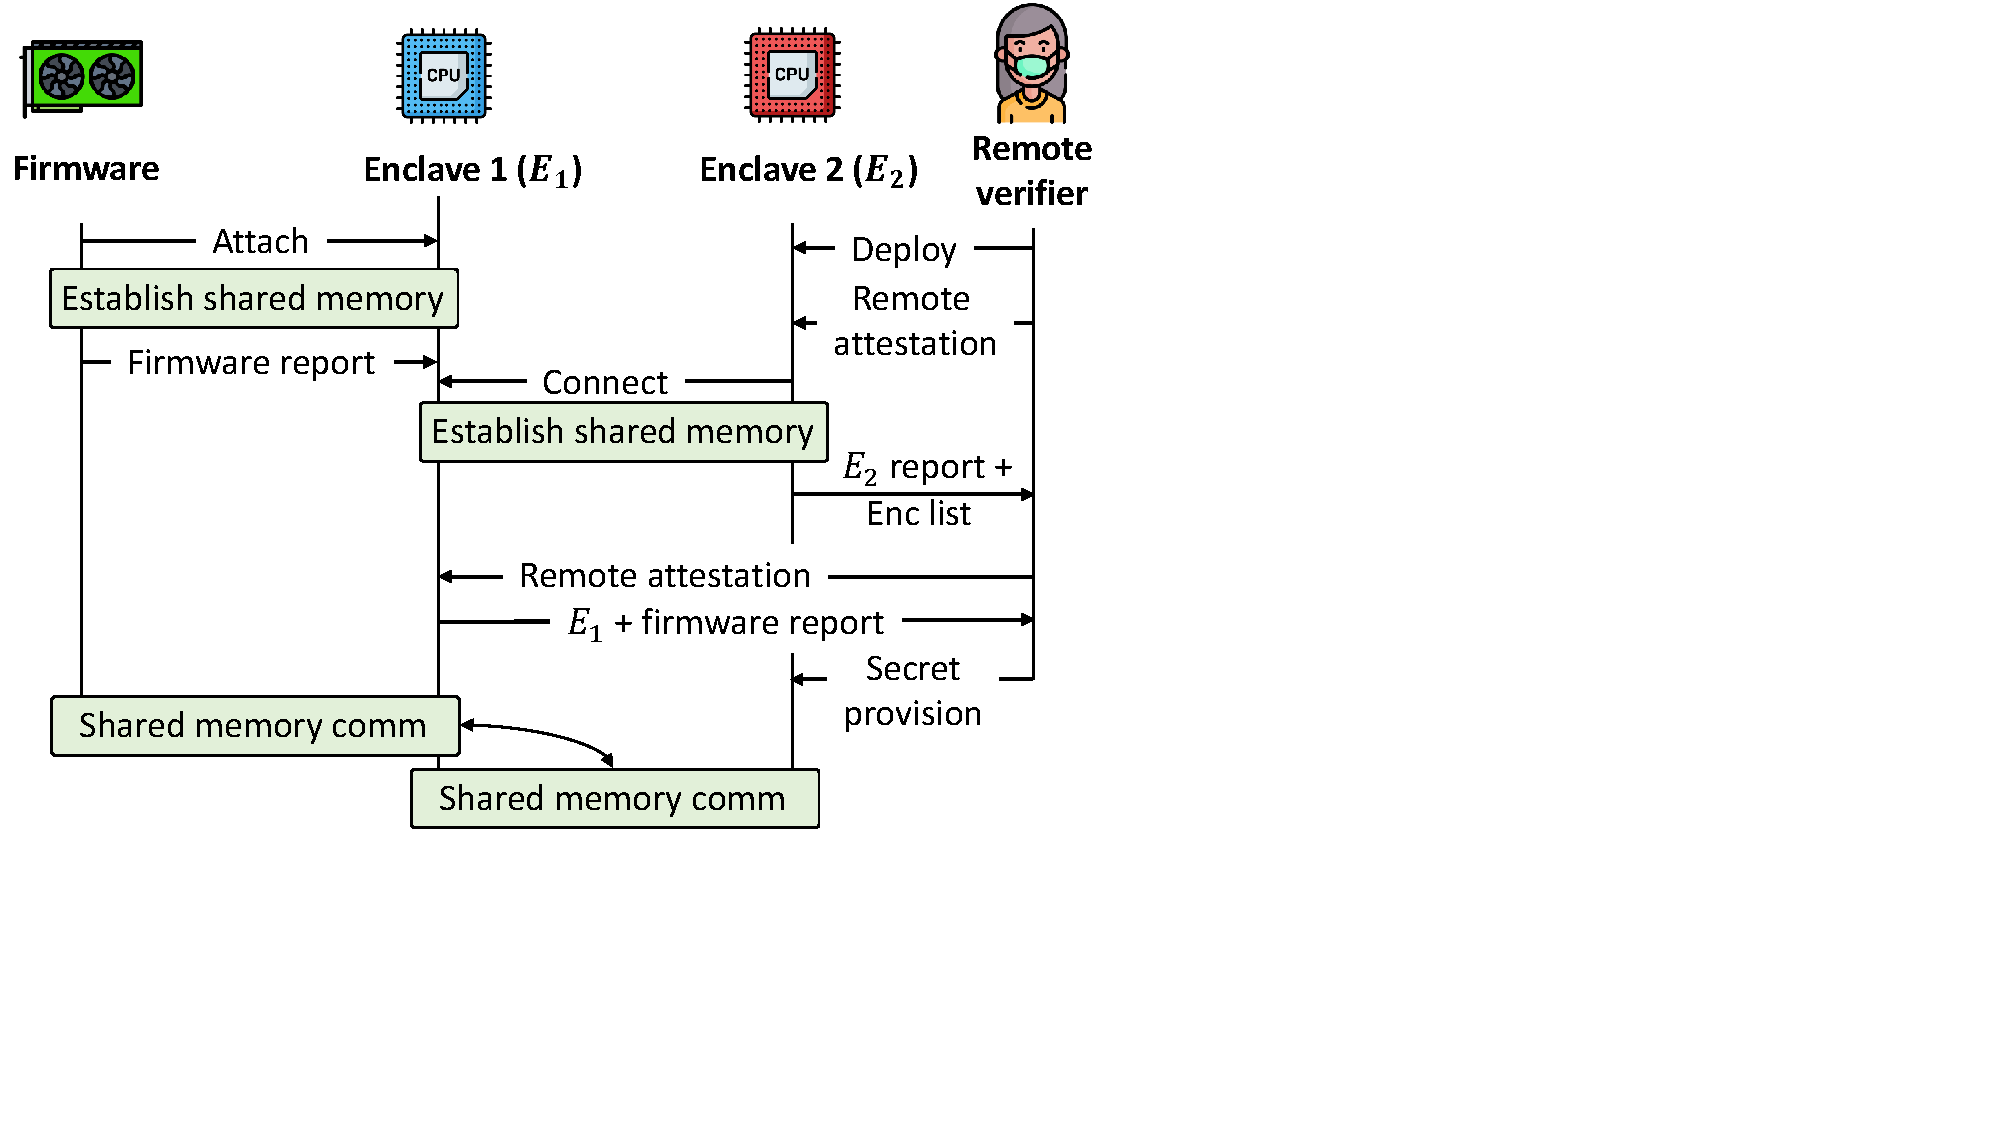
\includegraphics[trim={0 5cm 15cm 0}, clip, width=.8\linewidth]{chapters/PIE/images/localAttestation.pdf}
  \caption[Flow of (remote) platform-wide attestation process between \nameenclave{}'s components]{\textbf{Flow of the (remote) platform-wide attestation process} between the remote verifier, $E_1$, $E_2$ and the \sphw firmware. At the end of this process, the remote verifier receives the attestation report of $E_1$, $E_2$, and \sphw firmware, including their connection parameters such as DMA size, peripheral access control policy, etc.}   
  \label{fig:attestationFlow}
\end{figure}

\myparagraph{Attestation Flow}

Figure~\ref{fig:attestationFlow} depicts an example \nameenclave{} and the sequence of the attestations between its different components.The \name enclave contains three components \emph{enclave 1} ($E_1$), \emph{enclave 2} ($E_2$) and a \sphw firmware. Note that the platform-wide attestation process starts from the verifier who initiates a remote attestation request of $E_2$. 
The attestation report of $E_2$ includes a list  of connected enclaves' identifiers, notably $E_1$. The verifier then executes a series of individual remote attestation of all connected enclaves. Note that both individual attestations of $E_1$ and $E_2$ include each other's identifier in their list of connected components. Note that both the attestation reports of $E_1$ and $E_2$ are signed by the same platform key. This proves to the remote verifier that both the enclaves are running on the same platform.

For \sphw, the attestation mechanism is different. First of all, a \sphw needs to contain some key material and a signed certificate from the manufacturer. This allows a verifier to observe the legitimacy of the \sphw. Secondly, the verifier from \Cref{fig:attestationFlow} needs to be able to verify that the \sphw is directly talking to $E_1$. This is facilitated by the SM, who checks the address regions for MMIO registers. DMA regions can even be established by an untrusted entity such as the OS. However, the attestation report of both the \sphw and $E_1$ contains the physical memory region that they share.

